
%(BEGIN_QUESTION)
% Copyright 2010, Tony R. Kuphaldt, released under the Creative Commons Attribution License (v 1.0)
% This means you may do almost anything with this work of mine, so long as you give me proper credit

Suppose a particular 480 volt AC three-phase electrical system provides power to two induction motors:

$$\includegraphics[width=15.5cm]{i02186x01.eps}$$

Calculate the source's main line current feeding these two motors, assuming 100\% efficiency for each motor, and a perfect (1.0) power factor.

\vskip 50pt

Now calculate the source's main line current feeding these two motors, assuming 95\% efficiency for the small motor and 93\% efficiency for the large motor, and a perfect (1.0) power factor.

\underbar{file i02186}
%(END_QUESTION)





%(BEGIN_ANSWER)

Source line current (100\% efficiency) = 12.11 amps

\vskip 10pt

Source line current ($<$100\% efficiency) = 12.95 amps

%(END_ANSWER)





%(BEGIN_NOTES)

{\bf This question is intended for exams only and not worksheets!}.

%(END_NOTES)

